\section{Software}
I dette afsnit gennemgåes de forskellig dele af softwaren ved brug af flowcharts og psedokode.

\subsection{Generelt}
I dette projekt har vi skulle skrive en form for “OS” (Operating System) til vores kanontårn. Denne OS skal selvfølgelig stemme overens med opgavens krav. Den skal altså kunne bruges på et arduino chipset, samt være i stand til at afbryde handlinger baseret på input fra en controller-enhed.

\subsection{IDE og sprog}
Som sagt er der i projektet skrevet et program til et Arduino chipset. Selve programmet skal altså skrives i et sprog som Arduinoen kan forstå. I dette tilfælde er der skrevet i det Arduino dedikerede sprog, også kaldet Wire, som er en forgrening af de meget udbredte sprog “C” og “C++”\footnote{\url{ https://www.arduino.cc/en/Main/FAQ}}. Der er i projektet også brugt Arduinos egen basis IDE (Integrated Development Environment) da selve funktionerne og fejlfinding i dette projekt ikke har været problematisk nok til at kunne understøtte at bruge tid på at finde en udvidelse eller helt nyt udviklingsmiljø.

\subsection{Indsamling af viden om Arduino software}
I projektet har vi skulle bruge mange nye komponenter for at kunne opfylde de stillede krav. Dette har resulteret i, at det har været nødvendigt at søge ny information. Basis-principper vedrørende de nye komponenter er primært fundet fra siden “Sparkfun”\footnote{\url{https://learn.sparkfun.com/tutorials/using-the-BlueSMiRF/all }}, som har mange gode eksempler på både brug af komponenter og de mange forskellige måde som disse kan kobles til, og kommunikeres med gennem Arduino\footnote{Problemløsning med knapper:\url{https://www.arduino.cc/en/Tutorial/Button
}}. Udover denne hjemmeside har spørgsmålssegmentet på Arduinos egen hjemmeside ofte givet gode råd og har kunnet besvare spørgsmål med deres store forum.


\subsection{Program flow}
\begin{figure}[H]
\centering
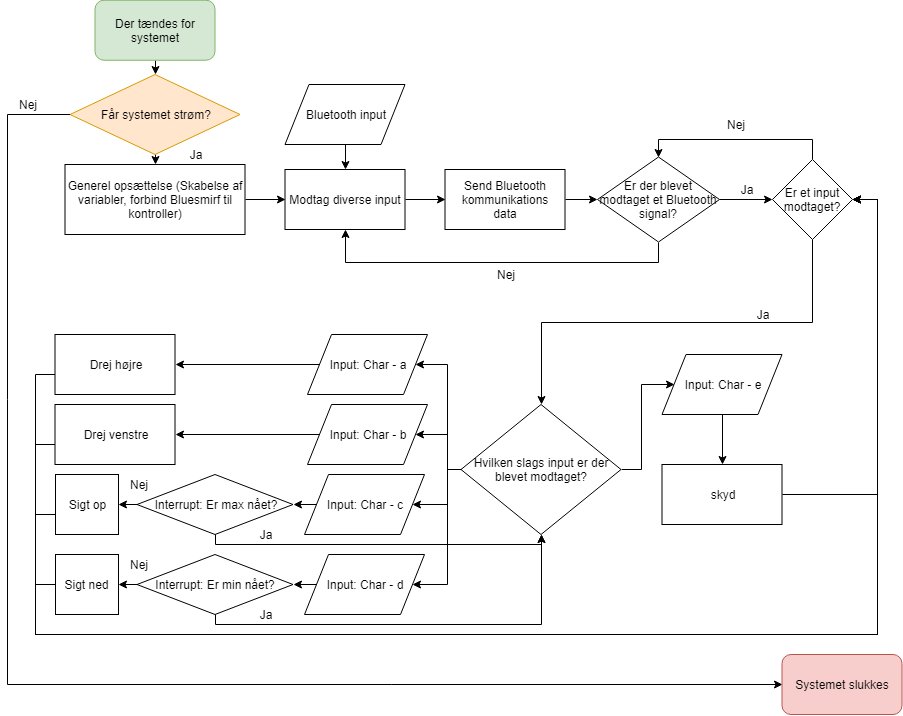
\includegraphics[scale=0.6,angle= 90]{Billeder/ProgramFlowchart.png}
\caption{Flowchart over softwarens logik.}
\label{fig:ProgramFlow}
\end{figure}

\subsection{Psedokode}
\subsubsection{Controller}
Oenskede biblioteker inkluderers, her bliver biblioteket “SoftwareSerial” inkluderet da dette skal bruges til seriel kommunikation mellem de to BlueSMiRF silver mates.\\

Foerst opsaettes Pins og globale vaerdier:\\
	//Nedenstaaende er pins som bruges til knapper\\
	KnapVenstre = 4\\
	KnapHojre = 5\\
	KnapOp = 6\\
	KnapNed = 7\\
	KnapSkyd = 8\\
	//Variabler til registreing af knaptryk\\
	KnapStateVenstre = 0\\
	KnapStateHojre = 0\\
	KnapStateOp = 0\\
	KnapStateNed = 0\\
	KnapStateSkyd = 0\\
	//Bluetooth pins til kommunikation oprettes\\
	BluetoothTx = 2\\
	BluetoothRx = 3\\

Herefter opsaettes “Void setup” hvor pins defineres til inten OUTPUT eller INPUT, og bluetooth kommonikations paabegyndes.\\
	Knap pins saettes til input\\
	Serial port startes ved standard baudrate paa 9600\\
	Bluetooth opstartes ved standard baudrate paa 115200\\
	Kommandosekvens paabegyndes.\\
	Naar kommandosekvensen har koert saettes baudraten ned fra 115200 til 9600\\ for ikke\\
	At skabe problemer med arduino kommunikation.\\
	Print “Ended Setup”\\

Der oprettes en boolsk vaerdi til at vurdere om kommandosekvens til opretelse af denne bluetoothenhed som master har koert.\\

Void loop:\\
	Der oprettes fem led i et elif statement til at sende fem kommando karaktere:\\
	Hvis knaptryk(a,b,c,d eller e):\\
		Send a,b,c,d eller e gennem bluetooth (korresponderende bogstav til knaptryk)\\
		Vent 250 millisekunder.\\
	Hvis bluetooth er tilgaengelig:\\
printes alle karaktere som er blevet sendt eller modtaget paa denne enheds serial  monitor.\\
	Ellers:\\
 printes der ikke noget.\\
 

\subsubsection{Turret}
Oenskede biblioteker inkluderers, her bliver biblioteket “SoftwareSerial” inkluderet da dette skal bruges til seriel kommunikation mellem de to BlueSMiRF silver mates.\\

Først opsaettes Pins og globale vaerdier:\\
	//Nedenstaaende er pins som bruges til at styre diverse dele af systemet:\\
	Hojre = 8 // 8 og 9 er til rotationsmotor\\
	venstre = 9\\
	Op = 10  // 10 og 11 er til at panorere op eller ned\\
	Ned = 11\\
	Skyd = 12 // pin 12 er til at skyde med\\
	LedPin = 13 // Til interrupt\\
	
	Volatile int state = LOW // Kontrol af led i interrupt, dette state er som standard LOW\\

	//Bluetooth pins til kommunikation oprettes\\
	BluetoothTx = 3\\
	BluetoothRx = 4\\

Herefter opsaettes “Void setup” hvor pins defineres til inten OUTPUT eller INPUT, og bluetooth kommonikations påbegyndes.\\
	Foerst startes seriel kommunikation ved en baudrate på 115200 som standard.\\
	Herefter initieres kommandosekvens.\\
	En kort pause for at sikre at mate’n sender cmd.\\
	Pins til kontrol saettes alle til OUTPUT.\\
Serial kommunikation startes ved standard baudrate på 9600 da 115200 kan vaere for  hurtigt til stabil kommunikation.\\
	Pins til motor og skud kontrol oprettes som OUTPUT.\\
	Interrupt oprettes til funktionen “blink” ud fra parameteren “state” og en aendring i state.\\
	Led Pin saettes til OUTPUT\\
$Interrupt standard pin INT0 saettes til “INPUT_PULLUP” som hiver interrupt segmentet frem i “stack”.$\\

Interrupt funktionen “Blink” oprettes:\\
	State = !state // her sker en aendring hvis et interrupt forekommer.\\

Void loop:\\
	Først sikres det at alle OUTPUT pins er LOW\\
	Hvis bluetooth er tilgaengelig:\\
		Opret switch statement med en case for hvert kommando tegn fra controleren,\\
		Altså a, b, c, d og e, som henholdsvis kontrolere en bestemt handling.\\


\subsection{Programbeskrivelse/gennemgang}
Selve Kanontårnets og controllerens OS er lavet i arduino til brug på både arduino UNO chipsæt og gruppens egen mikrocontroller. programmet indsamler data fra en sensor og flere forskellige knapper og bruger disse data til at bestemme tårnets handling.Hvis kanontårnet modtager en værdi baseret på et knaptryk fra controlleren vil tårnet udføre en af disse handlinger: Drej til højre, drej til venstre, panorer op, panorer ned og skyd. Hvis kanontårnet kommer til en max eller min værdi for geværets “hældning” registrere accelerometeret dette og bruger interrupt til at stoppe geværet fra at hæve eller sænke sig. Hvis ikke kanontårnet får noget input, eller ikke får noget bluetooth signal vil tårnet forholde sig í ro.





